\documentclass[letterpaper, 12pt]{article}
\usepackage[american]{babel}
\usepackage[utf8]{inputenc}
\usepackage[citestyle=apa,style=apa,backend=biber]{biblatex}
\usepackage[margin=1in]{geometry}
\usepackage{mathtools}
\DeclarePairedDelimiter\ceil{\lceil}{\rceil}
\DeclarePairedDelimiter\floor{\lfloor}{\rfloor}
\usepackage{caption}
\usepackage{float}
\usepackage{array}
\usepackage{verbatim}
\addbibresource{bibliography.bib}
\setlength\bibitemsep{2\itemsep}


\begin{document}
	\begin{titlepage}
		\centering
		\vspace*{5.75cm}
		{\huge\bfseries CIS 721\par}
		{\large RTOS, Raspberry Pi, and Sensor Interfacing\par}
		\vspace{2cm}
		Dan Wagner\\
		Kansas State University\\
		College of Engineering\\
		Department of Computer Science\\
		\vspace{1cm}
		Dr. Mitchell Neilsen\\
		Professor\\
		Department of Computer Science\\
		\vspace{1cm}
		May 8 2018
	\end{titlepage}

\section{Introduction}
A Raspberry Pi is a modular, advanced computing device that can be used in many projects.  It comes with 40 General Purpose Input/Output (GPIO) pins which can be attached to sensors, motors, and other similar devices \cite{raspberrypifoundation2018}.  By default, the Pi ships with the Raspian OS, which is a flavour of Debian Linux.  This OS is not a Real-Time OS (RTOS) but can be loaded with one (or a microkernel) on top of the existing system.  Once loaded with such software, code can be developed that allows for real-time constraints and modules.  In this project, the Xenomai 3 RTOS was installed on top of Raspbian to incorporate these characteristics.  Two sensors were attached to the system for real-time reporting: a DHT11 humidity/temperature sensor and a rotary encoder module.  Using the Xenomai 3 API, tasks were scheduled to periodically poll the sensors within specified deadlines.

The sections to follow will outline the project details.  First, the Xenomai 3 RTOS will be discussed, particularly outlining the functionality that is incorporated into the sensor software.  Second, the hardware specifications will be listed and discussed for the Raspberry Pi, rotary encoder, and DHT11.  Third, the software will be described in detail along with any design decisions.  Then, the project's results will be discussed and analyzed.  Finally, conclusions will be drawn from the previous discussions.
~\newline

\section{Xenomai 3}
Xenomai 3 is an RTOS developed by numerous engineers as an Free Software project for Linux machines (\cite{xenomai2018}).  It allowed for a versatile framework to be developed for real-time capabilities in Linux.  The RTOS provides an in-depth, detailed API for programmers to utilize when managing tasks.  In particular, several routines were used to create, initialize, schedule, and delete tasks. %(https://xenomai.org/documentation/xenomai-3/html/xeno3prm/group__alchemy__task.html#gababee94264156693cd4f5b9b70d3c5a1).
%Tasks were created using $rt\textunderscore task\textunderscore create()$.  This function informed Xenomai of a new task that needed to be created for later scheduling.  The name, priority, and 
~\newpage
\section{Hardware Specifications}
The Raspberry Pi 3B was used in this project; its relevant specifications are listed in the table below.  Its processor and RAM were more than capable of the project's requirements, and the numerous input/output pins allowed multiple sensors to be wired up.
~\newline
\begin{table}[hbt]
	\centering
	\caption{Raspberry Pi Specs}
	\label{my-label}
	\begin{tabular}{lllll}
		\cline{1-2}
		\multicolumn{1}{|l|}{Processor} & \multicolumn{1}{l|}{Quad Core 1.2GHz Broadcom BCM2837 64bit CPU} &  &  &  \\ \cline{1-2}
		\multicolumn{1}{|l|}{RAM} & \multicolumn{1}{l|}{1GB} &  &  &  \\ \cline{1-2}
		\multicolumn{1}{|l|}{Data Pins} & \multicolumn{1}{l|}{40 GPIO} &  &  &  \\ \cline{1-2}
		&                       &  &  & 
	\end{tabular}
\end{table}

Both sensors were distributed in a kit by Sunfounder.  The rotary encoder has a resolution 20 cycles per revolution, which means that twenty electrically high pulses will be present on the square wave per revolution (\cite{artofcircuits2018}).  

~\newline
The DHT11 recorded both humidity and temperature characteristics.  Both readings have a 16-bit resolution.  The sampling period is more than two seconds, and was the determining factor in the scheduling of tasks in Xenomai.

\begin{figure}[H]
	\centering
	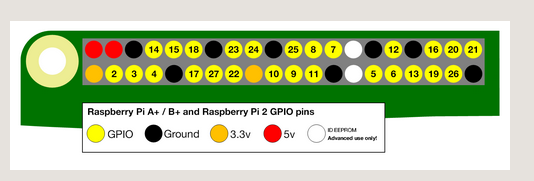
\includegraphics[width=10cm,height=10cm,keepaspectratio]{pi_GPIO.png}
	\caption[GPIO]{Pi 3 GPIO Pinouts. Courtesy of Raspberrypi.org.}
	\label{fig:GPIO}
\end{figure}

Above is an image that labels each numbered pin of the Raspberry Pi 3.
The rotary encoder required five pins: 5V, GND, Clock, Data, and Switch.  Pins 5V and GND were attached to the top row, second and third pins (red and black). Clock was wired to GPIO 16, Data to GPIO 27, and Switch to GPIO 22.  These pins were denoted by the hardware; as it will be discussed, in software, the pins were referred to by a different numbering mechanism.

~\newpage
The figure below shows the system's configuration.
Three pins were used for the DHT11: 5V, GND, and Data.  The 5V and GND signals were wired to the same pins as the rotary encoder through the use of a breadboard.  Data was wired to GPIO 23.  The following image shows the final setup of the system.

\begin{figure}[H]
	\centering
	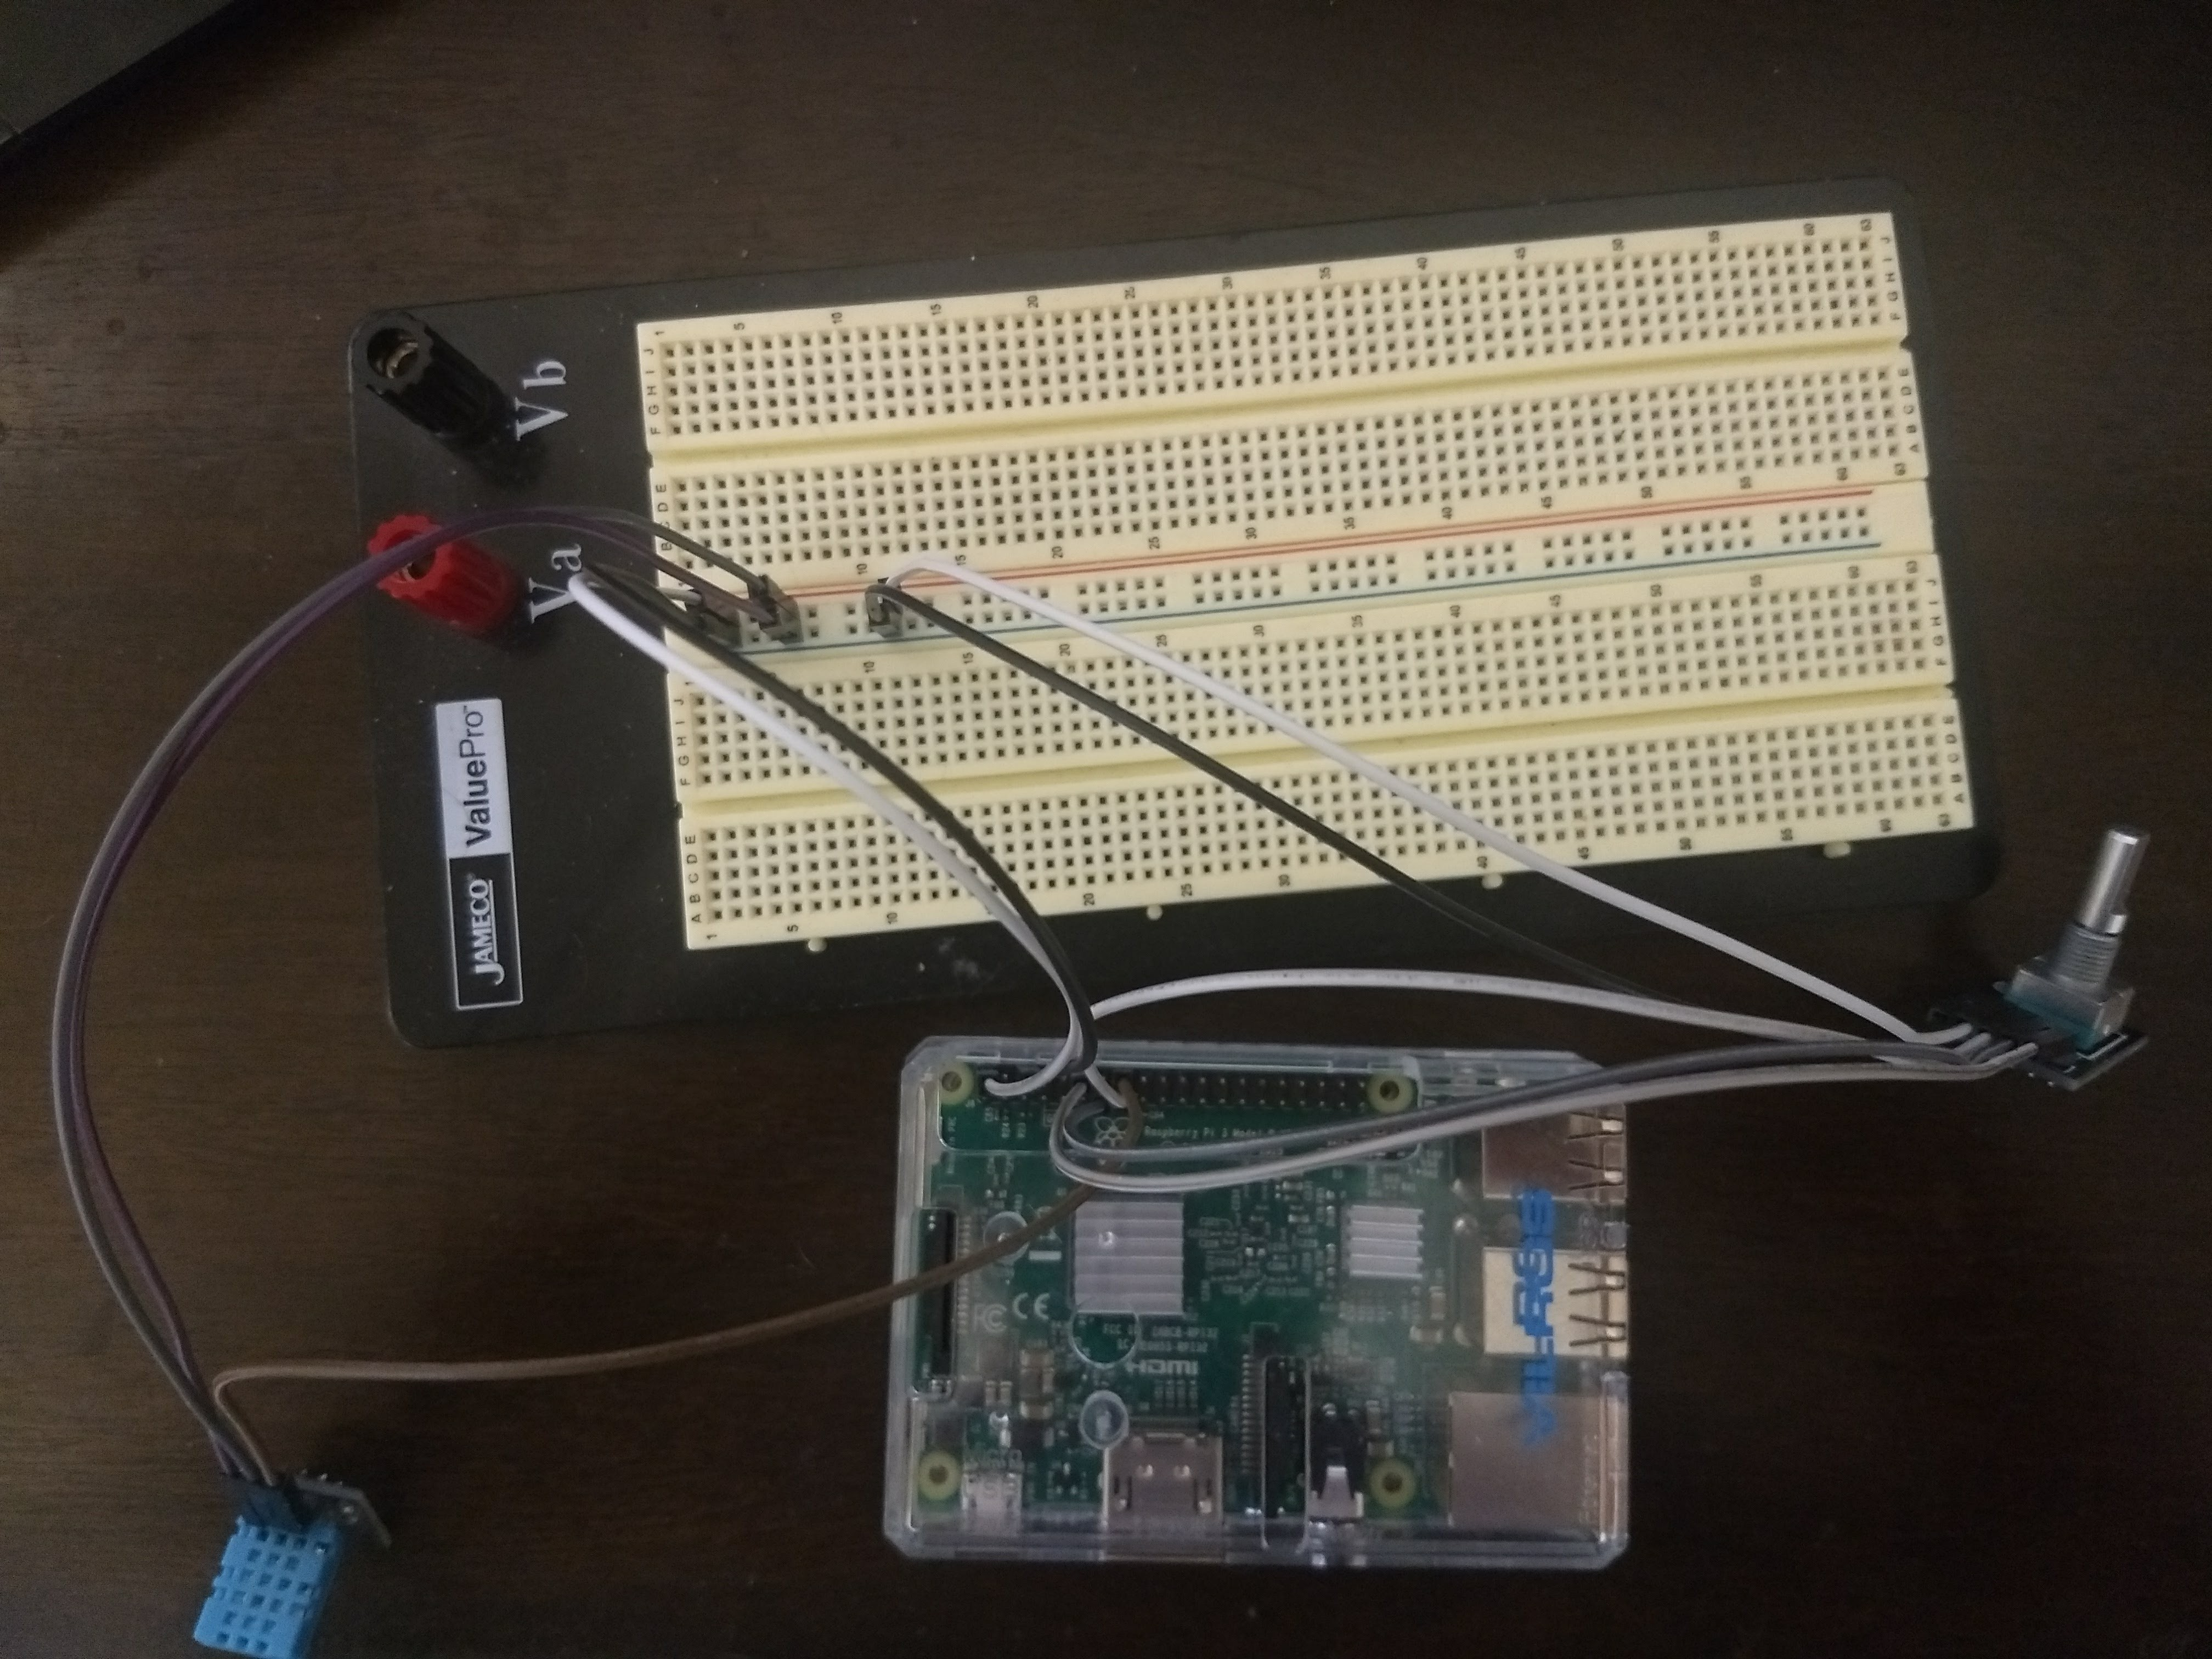
\includegraphics[width=10cm,height=10cm,keepaspectratio]{circuit.jpg}
	\caption[Ciruit]{Sensors and Pi Wiring.}
	\label{fig:Circuit}
\end{figure}
~\newline
% Module specs (latency, pulses, datasheets)
% Raspberry Pi specifications
% Photograph of connection information
\section{Software Specifications}
The system's real-time constraints were considered before any software was developed.  Sunfounder, the sensors' distributor, provided several code examples on their Github account to test each sensor (\cite{sunfounder2018}).  These constraints were derived from examining their source code.
  
\indent The DHT11 experienced high amounts of latency, as each reading required one second to be valid.  First, the sensor's pin was pulled low for 18ms. Then, it was pulled high for 40us in preparation to read the data.  After a slight delay from verifying the data's integrity via checksum, it was read, after which the next reading was not available for one second.  Any reduction in this delay caused a reading to be invalid, or missed.  As a result, failures of the DHT11 were defined as not receiving data from the sensor after one second.

\indent For the rotary encoder, the latency was very short.  From Sunfounder's source code, there was no delay explicitly defined.  After experimenting with the sensor, it was possible to retrieve information every 5ms without issue.  Thus, any failure of the encoder was defined as not recording a reading within five milliseconds.

\newpage
These real-time constraints were modeled in UPPAAL for verification.  Below is a visual representation of this model. 
\begin{figure}[H]
	\centering
	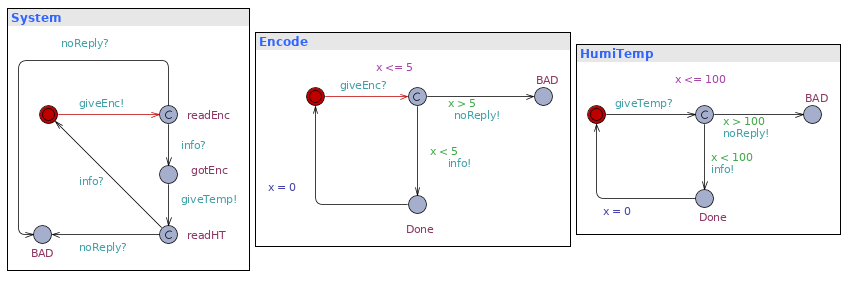
\includegraphics[width=10cm,height=10cm,keepaspectratio]{system.png}
	\caption[Model]{UPPAAL Model of the System.}
	\label{fig:model}
\end{figure}
One process represented the Raspberry Pi, with the encoder and DHT11 being additional processes.  First, the Raspberry Pi would request the encoder's data by signaling it along the giveEnc channel.  Upon receipt of this message, the encoder would enter an intermediate state with invariant of $x <= 5$; this modeled the latency in its operation.  If a fault occurred (i.e. $x == 5$), then a message on the noReply channel would be sent, the bad state would be entered and the Raspberry Pi would experience a failure.  Otherwise, the encoder sent data back to the Pi (via the info channel) and proceeded to a done state before resetting its local clock for the next request.  After receiving the encoder data, the Pi would ask the DHT11 for data by sending a message on the giveTemp channel.  The DHT11 functioned similarly to the encoder, but with a 1 second latency (100 time units).  If results were not available within one second, the sensor would report a fault on the noReply channel and enter a bad state.  Otherwise, it would send a reply on the info channel, enter a done state, and reset its local clock before awaiting the next poll from the Raspberry Pi.

\indent Three queries were used to verify these characteristics.  First, $E <> Encode.x > 5$ would test for a failure with the encoder.  Next, $E <> HumiTemp.x > 100$ would test for DHT11 failures.  Finally, $A[] not System.BAD and not Encode.BAD and not HumiTemp.BAD$ tested for a system failure, with both sensors failing within the same reading cycle.  UPPAAL's verifier returned that each of these queries were satisfied, so the system had no faults that could occur.

Once hardware connections were established and real-time constraints were verified, the software needed to interface with each device.  This was made possible using the WiringPi library (\cite{gordonhenderson2018}).  The GPIO designations in Figure \ref{fig:GPIO} were not the same as WiringPi used.  Figure \ref{fig:pinouts} shows these obvious differences. The software refers to each pin by its WiringPi number.  For the rotary encoder, the Clock, Data, and Switch pins were referred to as pins 1, 2, and 3 respectively.  The DHT11's Data pin was denoted as pin 4.  WiringPi used these numbers to interface with the Raspberry Pi through wiringPiSetup().  This function initialized the system to use its numbering scheme and allowed the data to be accessed on those pins.

\begin{figure}[H]
	\centering
	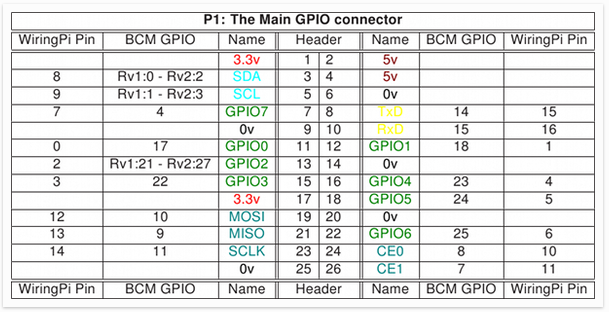
\includegraphics[width=10cm,height=10cm,keepaspectratio]{pi_pins.png}
	\caption[Pinouts]{WiringPi Pinouts. Courtesy of Wiringpi.com.}
	\label{fig:pinouts}
\end{figure}
~\newline

% UPPAAL model here
% Encoder ISR
% DHT11 ISR, checksum delay
% WiringPi
~\newpage
\section{Experimental Results}
~\newpage
\section{Conclusion}

~\newpage
\printbibliography
~\newpage
\section{Source Code}
\verbatiminput{project.c}

\end{document}